In this section, we describe our cross-protocol DROWN attack that uses an \ssltwo server as an oracle to efficiently decrypt TLS connections.  We first describe our techniques using a generic \ssltwo oracle.  In Section~\ref{vulnerability}, we show how a protocol flaw in \ssltwo can be used to construct such an oracle, and describe our general DROWN attack.  In Section~\ref{sec:special}, we show how an implementation flaw in common versions of OpenSSL leads to a very powerful oracle, and describe our efficient special DROWN attack.

%\subsection{An efficient Bleichenbacher attack}

\subsection{Attack scenario}
\label{sec:attack-scenario}

We consider a server that accepts TLS connections from clients. The connections are established using a secure, state-of-the-art TLS version (1.0--1.2) and a \texttt{TLS\_RSA} cipher suite where the private key is not known to the attacker.

\paragraph{Server RSA key exposed via \ssltwo.}
The same RSA public key as the TLS connections is also used for \ssltwo. 
\if0
This can arise in a number of situations that are common in practice.  The simplest case is a server (mis)configured to also support \ssltwo on the port accepting the TLS connections.  But the \ssltwo support may be on an entirely different port, or an entirely different server.
This situation might arise when an organization uses a wildcard certificate for both its website on port 443 and its SMTP server on port 25.  Both of these situations are common in practice; see Section~\ref{sec:scans} for more detail.  
\fi
For simplicity, our presentation will refer to the servers accepting TLS and \ssltwo connections as the same entity.

\paragraph{The attacker's position in the network.}
Our attacker is able to passively eavesdrop on traffic between the client and server and record RSA-based TLS traffic, but does not perform any active man-in-the-middle interference.
\ifext
The goal of our attacker is to decrypt a \texttt{TLS\_RSA} connection established between the server and one of the clients that connects to it.
Our attacker could be as sophisticated as a nation state with eavesdropping capabilities at Internet exchange points, or as simple as a neighbor on an open WiFi network.
\fi

The attacker can expect to decrypt one out of 1,000 intercepted TLS connections in our attack for typical parameters.  This is a devastating threat in many scenarios.  For example, a decrypted TLS connection might reveal a client's HTTP cookie or plaintext password, and an attacker would only need to successfully decrypt a single ciphertext to compromise the client's account.

In order to collect 1,000 TLS connections, the attacker might simply wait patiently until sufficiently many connections are recorded.  If the attacker's intended victim is the \emph{server}, rather than a specific client, observing this many connections from many clients might take only a short time for an attacker who is located at a company firewall or who could perform a DNS spoofing or BGP hijacking attack to redirect traffic transparently through themselves.  If the attacker's intended victim is a \emph{particular client}, this is still feasible in many cases.  As an example, the Mozilla Thunderbird email client will check for new email messages every ten minutes by default.  A targeted user will make 1,000 connections after leaving the application running for a week.  A less patient attacker could embed or inject malicious JavaScript on an otherwise innocuous web site to cause the client to connect repeatedly to the victim server in a short time frame, as in the BEAST attack~\cite{BEAST}.  Normally such connections would use TLS session resumption instead of completing a fresh handshake on each time, but if an attacker can trigger an error, the next connection will be negotiated with a fresh handshake.


\subsection{A generic \ssltwo oracle}

Our attacks make use of a padding oracle that can be queried on a ciphertext and leaks information about decrypted plaintext; this abstractly models the information gained from an \ssltwo server's behavior.  Our \ssltwo oracles reveal many bytes of plaintext, resulting in an efficient attack.

Our cryptographic oracle $\Oracle$ has the following functionality: 
$\Oracle$ decrypts an RSA ciphertext $c$ and responds with ciphertext validity based on the structure of the decrypted message $m$.  
The ciphertext is valid only if $m$ starts with \hexb{00}{02} followed by non-null padding bytes, a delimiter byte \hex{00}, and a \texttt{master\_key} $mk_{secret}$ of correct byte length $k$.
In the following, we denote such a ciphertext to be \textit{\sslconform}.

All of the \ssltwo padding oracles we instantiate give the attacker similar information about a \PKCSconform \ssltwo ciphertext:
\begin{equation*} 
\Oracle(c) =  
\begin{cases} 
mk_{secret} & \text{ if } c^d \bmod N = 00 || 02 || PS || 00 || mk_{secret}  \\ 
0 & \text{ otherwise.} 
\end{cases} 
\end{equation*}
That is, the oracle $\Oracle(c)$ will return the decrypted message $mk_{secret}$ if it is queried on a \PKCSconform \ssltwo ciphertext $c$ corresponding to a correctly \PKCS padded encryption of $mk_{secret}$.  The attacker then learns $k + 3$ bytes of information about $m = c^d \bmod N$: the first two bytes are $00 || 02$, and the last $k+1$ bytes are $00 || mk_{secret}$.  The length $k$ of $mk_{secret}$ varies based on the cipher suite used in the instantiation of the oracle.  For export-grade cipher suites such as \texttt{SSL\_RSA\_EXPORT\_WITH\_RC2\_CBC\_40\_MD5},
%or \texttt{SSL\_RSA\_EXPORT\_WITH\_RC4\_40\_MD5}\@,
$k$ will be 5 bytes, so the attacker learns 8 bytes of information about $m$. For 
%\texttt{SSL\_RSA\_WITH\_DES\_CBC\_SHA}\@, $k$ is 8 bytes; for 
\texttt{SSL\_DES\_192\_EDE3\_CBC\_WITH\_MD5}\@, $k$ is 24 bytes and the attacker learns 27 bytes of plaintext.

\subsection{DROWN attack template}
\label{sec:adapted-bb-compact}
Our attacker will use an \ssltwo oracle $\Oracle$ to decrypt a TLS \texttt{ClientKeyExchange}.  
The behavior of $\Oracle$ poses two problems for the attacker. First, a TLS ciphertext transmitted in a TLS key exchange decrypts to a 48-byte \pms. But since no \ssltwo cipher suites have 48-byte key strengths, this means that a valid TLS ciphertext is invalid to our oracle $\Oracle$. 
In order to apply Bleichenbacher's attack, the attacker needs to transform the TLS ciphertext into a valid \ssltwo key exchange message. Second, $\Oracle$ is very restrictive, since it strictly checks the length of the unpadded message. 
According to Bardou et al.~\cite{bardou2012efficient}, using such an oracle for Bleichenbacher's attack would require 12 million oracle queries.\footnote{See Table~1 in~\cite{bardou2012efficient}. The oracle is denoted with the term \texttt{FFF}.} 
%As each query would require an exhaustive search over $2^{40}$ values, this would make the attack significantly more costly.

Our attacker overcomes these problems by following this generic attack flow:
\begin{enumerate}
 \setcounter{enumi}{-1}
	\item The attacker collects many encrypted TLS RSA key exchange messages.
	\item He then attempts to convert the intercepted TLS ciphertexts containing a 48-byte \pms to valid RSA \PKCS encoded ciphertexts containing messages of length appropriate to the \ssltwo oracle $\Oracle$. We accomplish this by taking advantage of RSA ciphertext malleability and a technique of Bardou et al.~\cite{bardou2012efficient}.
	\item Once the attacker has obtained a valid \ssltwo RSA ciphertext, he can continue with a modified version of Bleichenbacher's attack, and decrypt the message after many more oracle queries.
	\item The attacker can then transform the decrypted plaintext back into the original plaintext, which is one of the collected TLS handshakes.
\end{enumerate}

We describe the algorithmic improvements we use to make each of these steps efficient below.

\subsubsection{Finding an \sslconform ciphertext}
\label{sec:trimmers}
The first step for the attacker is to transform the original TLS \texttt{ClientKeyExchange} message $c_0$ from a \tlsconform ciphertext into an \sslconform ciphertext. 
A trivial approach would be to generate multipliers $s_i \in \{s_1,s_2,\ldots\}$, and compute ciphertexts $c_i = (c_0 {s_i}^e) \bmod N$, until one gets accepted by $\Oracle$.
However, the number of generated ciphertexts would be high, because $\Oracle$ is very restrictive; for 2048-bit RSA keys and an oracle returning a 5-byte $k$ the probability that a random ciphertext becomes \sslconform is $P_{rnd} \approx (1/256)^3 * (255/256)^{249} \approx 2^{-25}$.

Instead, we rely on the concept of \emph{trimmers}, which were introduced by Bardou et al.~\cite{bardou2012efficient}. 
Assume that the message $m_{0} = {c_0}^d \bmod N$ is divisible by a small number~$t$. In that case,  $m_{0} \cdot t^{-1} \bmod{N}$ simply equals the natural number $m_{0} / t$. 
If we choose $u \approx t$, and multiply the original message with a fraction $u/t$, the resulting number will lie near the original message: $m_0 \approx m_0 / t \cdot u$.   We shall refer to such fractions as ``small'' fractions.

This method allows us to generate new \sslconform messages with a much higher probability. 
Let $c_0$ be an intercepted \tlsconform RSA ciphertext, and let $m_0 = c_0^d \bmod N$ be its corresponding plaintext.  We select a multiplier $s = u/t \bmod N = u t^{-1} \bmod N$ where $u$ and $t$ are coprime, compute the value $c_1 = c_0 s^e \bmod N$, and query $\Oracle(c_1)$.  We will receive a response if $m_1 = m_0 \cdot u/t$ is \sslconform.  

As an example, let us assume a 2048-bit RSA ciphertext with $k = 5$, and consider the fraction $u = 7, t = 8$.  The probability that a random ciphertext $c_0$ will be \sslconform is 1/7,774, so we expect to make 7,774 oracle queries before discovering a ciphertext $c_0$ for which $c_0 u/t$ is \sslconform, much better than a randomly selected multiplier. Appendix~\ref{sec:fraction-probability} gives more details on computing these probabilities.

\subsubsection{Shifting known plaintext bytes}
\label{sec:rotations}
Once we have obtained an \sslconform ciphertext $c_1$, we have also learned from our oracle information about the $k+1$ least significant bytes ($mk_{secret}$ together with the delimiter byte \hex{00}) and two most significant \hexb{00}{02} bytes of the \sslconform message $m_1$.  We would like to \emph{rotate} these known bits around to the right, so that we have a large block of contiguous known most significant bytes of plaintext.
In this section, we show that this can be accomplished by multiplying by some shift $2^{-r} \bmod N$.  In other words, given an \sslconform ciphertext $c_1 = m_1^e \bmod N$, we can efficiently generate an \sslconform ciphertext $c_2 = m_2^e \bmod N$ where $m_2 = s \cdot m_1 \cdot 2^{-r} \bmod N$ and we know several most significant bytes of $m_2$. 

Let $R = 2^{8(k+1)}$ and $B = 2^{8(\ell-2)}$. Abusing notation slightly, let the integer $m_1 = 2 \cdot B + PS \cdot R + mk_{secret}$ be the plaintext satisfying $m_1^e = c_1 \bmod N$.  At this stage, the $k$-byte integer $mk_{secret}$ is known and the $\ell-k-3$-byte integer $PS$ is not.

Let $\tilde{m_1} = 2 \cdot B + mk_{secret}$ be the known components of $m_1$, so $m_1 = \tilde{m_1} + PS \cdot R$. We can use this to compute a new plaintext for which we know many most significant bytes.  Consider the value 
\[
m_1 \cdot R^{-1} \bmod N = \tilde{m_1} \cdot R^{-1} + PS \bmod N.
\]
The value of $PS$ is unknown, but we know that it consists of $\ell-k-3$ bytes.  This means that the known value $\tilde{m_1} \cdot R^{-1}$ shares most of its $k+3$ most significant bytes with $m_1 \cdot R^{-1}$.

Furthermore, we can iterate this process by finding a new multiplier $s$ such that $m_2 = s \cdot m_1 \cdot R^{-1} \bmod N$ is also \sslconform.  A randomly chosen $s < 2^{30}$ will work with probability $2^{-25.4}$.  We can take advantage of the bytes we have already learned about $m_1$ to efficiently compute such an $s$ with only 678 oracle queries in expectation for a 2048-bit RSA modulus.   Appendix~\ref{sec:rotation-details} gives more details.

\subsubsection{Adapted Bleichenbacher iteration}
\label{sec:bb-iteration}
It is feasible for all of our oracles to use the previous technique to entirely recover a plaintext message.  However, for our \ssltwo protocol oracle it is cheaper to continue using Bleichenbacher's original attack, once we have used the above techniques to obtain a \sslconform message $m_3$ and an integer $s_3$ such that $m_3 \cdot s_3$ is \sslconform.  At this point, we can apply the original algorithm proposed by Bleichenbacher as described in Section~\ref{sec:bleichenbacher}, with minimal modifications.

Each step obtains a message that starts with the required \hexb{00}{02} bytes after two queries in expectation.
Since we know the value of the $k+1$ least significant bytes after multiplying by any integer, we can query the oracle only on multipliers that cause the $(k+1)$st least significant byte to be zero.  However, we cannot ensure that the padding string is entirely nonzero; for a 2048-bit modulus this will hold with probability 0.37.

For a 2048-bit modulus, the total expected number of queries when using this technique to fully decrypt the plaintext is $2048 * 2 / 0.37 \approx 11,000$.


\section{General DROWN} 
\label{vulnerability}

In this section, we describe how any correct \ssltwo implementation that accepts export-grade cipher suites can be used as a padding oracle.  We then show how to adapt the techniques described in Section~\ref{sec:adapted-bb-compact} to decrypt TLS RSA ciphertexts.

\subsection{The SSLv2 export padding oracle} 
\label{vulnerability}
\ssltwo is vulnerable to a direct message side channel vulnerability exposing a Bleichenbacher oracle to the attacker.
The vulnerability follows from three properties of \ssltwo.  First, the server immediately responds with a \texttt{ServerVerify} message after receiving the \texttt{ClientMasterKey} message, which includes the RSA ciphertext, without waiting for the \texttt{ClientFinished} message that proves the client knows the RSA plaintext.  Second, when choosing 40-bit export RC2 or RC4 as the symmetric cipher, only 5 bytes of the \texttt{master\_key} ($mk_{secret}$) are sent encrypted using RSA, and the remaining 11 bytes are sent in cleartext.  Third, a server
implementation that correctly implements the anti-Bleichenbacher countermeasure 
and receives an RSA key exchange message with invalid
padding will generate a random premaster secret and carry out the
rest of the TLS handshake using this randomly generated key material.

This allows an attacker to deduce the validity of RSA ciphertexts in the following manner:

\begin{enumerate}
	\item The attacker sends a \texttt{ClientMasterKey} message, which contains an RSA ciphertext $c_0$ and any sequence of 11 bytes as the clear portion of the \texttt{master\_key}, $mk_{clear}$. The server responds with a \texttt{ServerVerify} message, which contains the \texttt{challenge} encrypted using the \texttt{server\_write\_key}.
	\item The attacker performs an \textit{exhaustive search} over the possible values of the 5 bytes of the \texttt{master\_key} $mk_{secret}$. He then computes the corresponding \texttt{server\_write\_key} and checks whether the \texttt{ServerVerify} message decrypts to the \texttt{challenge}. One value should pass this check; let this value be termed $mk_0$. Recall that if the RSA plaintext was valid, $mk_0$ is the unpadded data in the RSA plaintext. Otherwise, $mk_0$ is a randomly generated sequence of 5 bytes.
	\item The attacker re-connects to the server with the same RSA ciphertext $c_0$. The server responds with another \texttt{ServerVerify} message that contains the current \texttt{challenge} encrypted using the current \texttt{server\_write\_key}. If the decrypted RSA ciphertext was valid, the attacker can directly decrypt a correct \texttt{challenge} value from the \texttt{ServerVerify} message by using the \texttt{master\_key} $mk_0$. Otherwise, if the \texttt{ServerVerify} message does not correctly decrypt to the \texttt{challenge}, the RSA ciphertext was invalid, and the attacker knows the $mk_0$ value was generated at random.
\end{enumerate}

Thus we can instantiate an oracle $\OracleSSLexp$ using the procedure above; each oracle query requires two server connections and $2^{40}$ decryption attempts in the simplest case.  For each oracle call $\OracleSSLexp(c)$, the attacker learns whether $c$ is valid, and if so, learns the two most significant bytes \hexb{00}{02}, the sixth least significant \hex{00} delimiter byte, and the value of the 5 least significant bytes of the plaintext $m$.

If the server does not support 40-bit export ciphers, the attack can also be mounted in feasible computation time by choosing DES as the symmetric cipher.  Choosing DES means the exhaustive search is now done over a key space of 56 bits, thus increasing the cost of the attack by a factor of \begin{math} 2^{16} \end{math}, but does not fundamentally change anything except the increased cost.

\ifsubmit\relax\else
\subsection{OpenSSL special DROWN oracle}

We discovered a vulnerability present in OpenSSL versions prior to March 4, 2015 that allows a client to improperly provide cleartext key bytes for non-export ciphers.  Affected servers will substitute these bytes for bytes from the encrypted key.  This allows a client to successively learn a byte at a time of an encrypted key by brute forcing only 256 possibilities for each query. For a non-export 128-bit cipher suite such as \texttt{SSL\_RC4\_WITH\_MD5}, the attacker learns 19 bytes of the decrypted message.  We describe this vulnerability in more detail in Appendix~\ref{sec:clear-key-vuln}.  A client can then construct a Bleichenbacher oracle from this behavior by validating the \texttt{ServerVerify} message against the candidate key provided in the \texttt{clear\_key\_data}, resulting in no brute-force computation.
\fi

\begin{figure}[t]
	%\centering 
	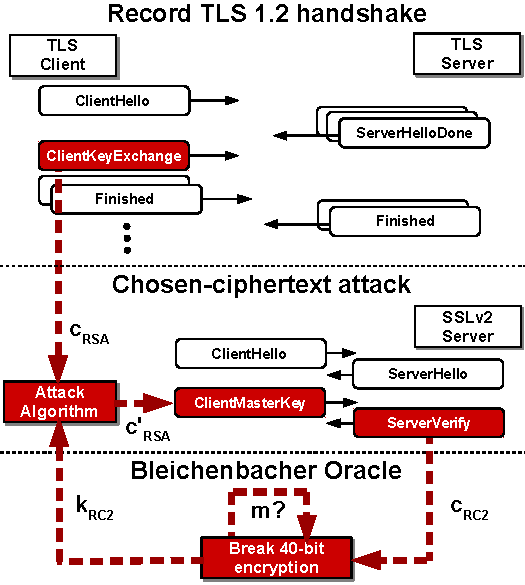
\includegraphics[width=\linewidth]{img/ssl-tls} 
	\caption{\textbf{Our \ssltwo-based Bleichenbacher attack on TLS\@.} An attacker passively collects RSA ciphertexts from a TLS 1.2 handshake, and then performs oracle queries against a server that supports \ssltwo with the same public key to decrypt the TLS ciphertext.}
	\label{fig:ssl-tls}
\end{figure}

\subsection{TLS decryption attack}

In this section, we describe how the oracle described in Section~\ref{vulnerability} can be used to carry out a feasible attack to decrypt passively collected TLS ciphertexts.

\subsubsection{Attack scenario}
As described in Section~\ref{sec:attack-scenario}, we consider a server that accepts TLS connections from clients using an RSA public key that is exposed via \ssltwo, and an attacker who is able to passively observe these connections.

\paragraph{Server supports export cipher suites for \ssltwo.}
We also assume the server supports export cipher suites for \ssltwo.
This can happen for two reasons.
First, the same servers that fail to follow best practices in disabling \ssltwo~\cite{ProhibitingSSLv2} may also fail to follow best practices by supporting export cipher suites.
Alternatively, the servers might be running a version of OpenSSL prior to January 2016, in which case they are vulnerable to the OpenSSL cipher suite selection bug described in Section~\ref{sec:openssl-selection}, and an attacker may negotiate a cipher suite of his choice independent of the server configuration.

\paragraph{Correct Bleichenbacher countermeasure.}
We assume the server implements the recommended countermeasure against Bleichenbacher's attack in all protocol versions, including \ssltwo. If the decrypted RSA ciphertext has invalid padding, the server generates a random \pms or \texttt{master\_key} and continues the handshake with this random string. We assume this countermeasure is implemented correctly and the server is neither vulnerable to timing nor flush-and-reload side-channel attacks~\cite{Meyer14,Zhang:2014:CSA:2660267.2660356}.

\paragraph{Computing power.}
The attacker needs access to computing power sufficient to perform a $2^{50}$ time attack, mostly brute forcing symmetric key encryption.  After our optimizations, this can be done with a one-time investment of a few thousand dollars of GPUs, or in a few hours for a few hundred dollars in the cloud.  Our cost estimates are described in~Section~\ref{sec:ec2_results}.

\if0
In our simplest attack scenario, an attacker is passively observing many connections between modern clients and server who negotiate a secure TLS version (1.0--1.2) with an RSA cipher suite and a well-generated, secure RSA public key.   The server is also configured to support \ssltwo with the same certificate as in TLS if a client requests it, although the modern victim clients will never negotiate \ssltwo.  The server implements the recommended countermeasures against Bleichenbacher attacks described in Section~\ref{sec:bleichenbacher}.



Our attacker will use our SSLv2 oracle $\OracleSSL$ to decrypt a TLS \texttt{ClientKeyExchange}.  We specialize the discussion below to our protocol-level oracle described in Section~\ref{vulnerability} and refer to this attack as the \emph{general} DROWN attack.  The adaptations to the OpenSSL clear-key oracle, which produces our faster \emph{special} DROWN attack are similar and are described in Section~\ref{sec:special}.
\fi

\subsubsection{Constructing the attack}

The attacker can exploit the \ssltwo vulnerability as illustrated in Figure~\ref{fig:ssl-tls}, following the generic attack outline described in Section~\ref{sec:adapted-bb-compact} and has several distinct phases:
\begin{enumerate}
 \setcounter{enumi}{-1}
	\item He passively collects 1,000 TLS handshakes from connections using RSA key exchange.
	\item The attacker then attempts to convert the intercepted TLS ciphertexts containing a 48-byte \pms to valid RSA \PKCS encoded ciphertexts containing five-byte messages using the fractional trimmers described in Section~\ref{sec:trimmers}, and querying $\OracleSSLexp$. The attacker sends the modified ciphertexts to the server using fresh \ssltwo connections with weak symmetric ciphers and uses the \texttt{ServerVerify} messages to deduce ciphertext validity as described in the previous section. For each queried RSA ciphertext, the attacker must perform a brute force attack on the weak symmetric cipher. The attacker expects to obtain a valid \ssltwo ciphertext after roughly 10,000 oracle queries, or 20,000 connections to the server.
	\item Once the attacker has obtained a valid \ssltwo RSA ciphertext $m_1$, he uses the shifting technique explained in Section~\ref{sec:rotations} to find an integer $s_1$ such that $m_2 = m_1 \cdot 2^{-40} \cdot s_1$ is also \sslconform.  Appendix~\ref{sec:general-rotations} contains more details on this step.
	\item The attacker then applies the shifting technique again to find another integer $s_2$ such that
		$m_3 = m_2 \cdot 2^{-40} \cdot s_2$ is also \sslconform.
	\item He then searches for yet another integer $s_3$ such that $m_3 \cdot s_3$ is also \sslconform.
	\item Finally, the attacker can continue with our adapted Bleichenbacher iteration technique described in Section~\ref{sec:bb-iteration}, and decrypts the message after an expected 10,000 additional oracle queries, or 20,000 connections to the server.
	\item The attacker can then transform the decrypted plaintext back into the original plaintext, which is one of the 1,000 intercepted TLS handshakes.
\end{enumerate}

\paragraph{The rationale behind the different phases.}
Bleichenbacher's original algorithm requires a conformant message $m_0$, and a multiplier $s_1$ such that $m_1 = m_0 \cdot s_1$ is also conformant.
Na\"{\i}vely, it would appear we can apply the same algorithm here, after completing Phase 1.
However, the original algorithm expects $s_1$ to be of size about $2^{24}$. This is not the case when we use fractions for $s_1$, as the integer $s_1 = u t^{-1} \bmod N$ will be the same size as $N$.

Therefore, our approach is to find a conformant message for which we know the 5 most significant bytes; this will happen after multiple rotations and
this message will be $m_3$.
After finding such a message, finding $s_3$ such that $m_4 = m_3 \cdot s_3$ is also conformant becomes trivial.
From there, we can finally apply the adapted Bleichenbacher iteration technique as described in Appendix~\ref{sec:general-bleichenbacher}.

\begin{table}[t]
  \centering
	\begin{tabular}{rrrrrr}
	\toprule
	\textbf{Optimizing} & \textbf{Cipher-} & \textbf{$|F|$}     & \textbf{\ssltwo}  & \textbf{Offline} \\
        \textbf{for}        & \textbf{texts}   &           & \textbf{connections} & \textbf{work} \\
	\midrule
	offline work        &           12,743 &          1 &            50,421  & $2^{49.64}$ \\
        offline work        &            1,055 &         10 &              46,042  & $2^{50.63}$ \\
	% compromise is achieved by using fractions {8/7, 8/9}; numbers are now final
       	compromise          &            4,036 &          2 &              41,081  & $2^{49.98}$ \\
	online work         &            2,321 &          3 &              38,866  & $2^{51.99}$ \\
	online work         &              906 &          8 &              39,437  & $2^{52.25}$ \\
	\bottomrule
	\end{tabular}
        \caption{\textbf{2048-bit Bleichenbacher attack complexity.} The cost to decrypt one ciphertext can be adjusted by choosing the set of fractions $F$ the attacker applies to each of the passively collected ciphertexts in the first step of the attack. This choice affects several parameters: the number of these collected ciphertexts, the number of connections the attacker makes to the \ssltwo server, and the number of offline decryption operations.}% The number of connections for the remaining phases after phase 1 is roughly 24,936, independently of phase 1.}
        \label{tab:reasonable_parameters}
\end{table}

\begin{table}[t]
\begin{tabular*}{\linewidth}{@{\extracolsep{\fill}\hskip\tabcolsep}rrrrr}
\toprule
\textbf{Key size}    & \textbf{Phase 1} & \textbf{Phases 2--5} & \textbf{Total}   & \textbf{Offline} \\
                     &                 &                 & \textbf{queries} & \textbf{work}    \\
\midrule
% This is all when using 4/5, which has a maximal "native probability" of 0.1.
% Offline work is always step1 * 2**38
%              1024 &  (0.1 * 0.62 * 1/256)**(-1)  & + 256 / 0.62 * 2 + 2/0.62 + 1024 * 2 / 0.62
               1024 &  4,129   &  4,132  &  8,261 & $2^{50.01}$ \\

%              2048 & (0.1 * 0.37 * 1/256)**(-1)   & + (2.72 * 2**8) * 2 + 2.72*2 + 2048 * 2 / 0.37 (number for phase 5 also matches runs)
               2048 &  6,919   &  12,468 & 19,387 & $2^{50.76}$ \\

%              4096 & (0.1 * 0.14 * 1/256)**(-1)   & + 2**8 / 0.14 * 2 + 2/0.14 + 4096 * 2 / 0.14
               4096 &  18,286  &  62,185 & 80,471 & $2^{52.16}$ \\
\bottomrule
\end{tabular*}
\caption{\textbf{Oracle queries required by our attack.} In Phase 1, the attacker queries the oracle until an \ssltwo conformant ciphertext is found.  In Phases 2--5, the attacker decrypts this ciphertext using leaked plaintext.  These numbers minimize total queries.  In our attack, an oracle query represents two server connections.}
\label{tab:optimal_queries}
\end{table}

\newcommand{\GPUTable}{
\begin{table*}[t]
 \centering
 \begin{tabular}{llrrrr}
        \toprule
        \textbf{Platform} & \textbf{Hardware} & \textbf{Cost} & \textbf{Full attack}  & \textbf{Cost to perform attack in 1 day} \\
        \midrule
        Na\"{\i}ve CPU & 4 Intel Xeon E7-4820 & $\$21,400$ & $114$ days  & \$$2,440,000$\\
        Na\"{\i}ve GPU & ZOTAC GeForce GTX TITAN & $\$2,400$  & $189$ days & \$$450,000$ \\
        Na\"{\i}ve FPGA & 64 Spartan-6 LX150 & $\$60,000$ & $51.5$ days  & \$$3,090,000$  \\
        \cmidrule{1-5}
        Optimized Hashcat & NVIDIA GTX / AMD R9 & \$18,040 & $0.75$ days & \$13,500 \\
        Optimized EC2 & NVIDIA & \$440 & $0.33$ days & \$147 \\
        \bottomrule
  \end{tabular}	
\caption{\textbf{Time and cost efficiency of our attack on different hardware platforms.} The brute force attacks against symmetric export keys are the most expensive part of our attack.  We compared the performance of a na\"{\i}ve implementation of our attack on different platforms, and decided that a GPU implementation held the most promise.  We then heavily optimized our GPU implementation, obtaining several orders of magnitude in speedup.}
\label{perf_comparison}
\end{table*}
}

\subsubsection{Attack performance}
\label{sec:bb-performance}
The attacker wishes to minimize three major costs in the attack: the number of recorded ciphertexts from the victim client, the number of connections to the victim server, and the number of symmetric keys to be brute forced.
The requirements for each of these elements are governed by the set of fractions to be multiplied with each RSA ciphertext in the first phase, as described in Section~\ref{sec:trimmers}.

Table~\ref{tab:reasonable_parameters} highlights a few choices for $F$ and the resutling performance metrics for 2048-bit RSA keys.
Appendix \ref{sec:general-performance} provides more details on the derivation of these numbers and other possible optimization choices.
Table \ref{tab:optimal_queries} gives the expected number of Bleichenbacher queries for different RSA key sizes, when minimizing total oracle queries.

%These are fractions of small coprime numbers, similar to the example $u/t = 8/7$, and ideally amenable to the additional optimization described above.





%The special DROWN attack requires similar numbers of ciphertexts and oracle queries, but the amount of computation is negligible.

